%SourceDoc ../YourName-Dissertation.tex
\vspace*{-80mm}
\chapter{Uniform Heating Problem} \label{chapter5:uniform_heating1}
 
\section{Problem Setup}

%Round off error, iterative convergence error.
%Discretization error?? (Check with)

The test problem is a nuclear rod with uniform heat generation with parameters
given in Table \ref{table:heating:parameters}. The fuel and cladding are assumed
to have constant material properties. The mass flow rate, reference pressure, and inlet
temperature approximate normal PWR operating conditions. However, the heat
generation rate is much less than normal PWR operating conditions to ensure that
the problem remains well  within the single-phase regime with an expected outlet
temperature of under 300.0 $^{\circ}C$. Additionally, the problem is set
up so that the calculation of the heat transfer coefficient using the Dittus-Boelter
correlation is appropriate. The subchannel is rod centered with no grid spacers
or frictional losses. Gravity pressure losses in the vertical direction are
taken into account. 

\begin{table}[h]
\center
\caption{Problem Parameters}
\label{table:heating:parameters}
\begin{tabular}{|c|c|c|c|}
\hline
Parameter			&	Symbol	&	Value	&	Unit	\\ \hline
Mass Flow Rate 		& $\dot{m}$ &   0.300   &   $\frac{kg}{sec}$  \\ \hline
Pressure			&	$P_{o}$	&	165.00	&	bar	\\ \hline
Inlet Temperature	&$T_{inlet}$&	290.00	&	$^{\circ}$C	\\ \hline
Linear Heat  Rate	& $q'$  	& 	4.00 	& $\frac{kW}{m-rod}$ \\ \hline
Active Fuel Length 	& $L$		& 	3.658	& $m$	\\ \hline
Fuel Radius	& $r_{fuel}$ & 0.4096 & $cm$ \\ \hline
Outer Cladding Radius &	$r_{co}$ & 	0.475	& $cm$ \\ \hline
Inner Cladding Radius & $r_{ci}$ &	0.4174	& $cm$ \\ \hline
Rod Pitch	& $p$ &	12.60	& $cm$ \\ \hline
Clad Specific Heat	& $c_{p,clad}$	& 0.431&  $\frac{kJ}{kg-K}$ \\ \hline
Clad Density & $\rho_{clad}$ &	8470.57 & $\frac{kg}{m^{3}}$ \\ \hline
Clad Thermal Conductivity & $k_{clad}$ & 14.83 & $\frac{W}{m-k}$ \\ \hline
Fuel Specific Heat Capacity & $c_{p,fuel}$ & 0.289 & $kJ/kg-K$ \\ \hline
Fuel Density & $\rho_fuel$ & 10970.40 & $\frac{kg}{m^{3}}$ \\ \hline
Fuel Thermal Conductivity & $k_fuel$ & 14.83 & $\frac{W}{m-k}$ \\ \hline
Gap Heat Transfer Coefficient & $h_{gap}$ & 5678.30	& $\frac{W}{m^2-K}$ \\
\hline
\end{tabular}
\end{table}

\section{Steady State Analytical Solution}

At steady state conditions and for uniform heat generation, the original
conduction equation can be integrated to obtain equation \ref{eq:uheat:fuel} for
$0.0 \leq r < r_{fuel}$.

\begin{equation}
	\label{eq:uheat:fuel}
	T_{rod}(r,z)-T_{rod}(r_{fuel},z)
	=\frac{q''' r_{fuel}^{2}}{4 k_{fuel}}\left(1-\frac{r^{2}}{r_{fuel}^{2}}\right)
\end{equation}

The temperature at the fuel surface can be calculated from the cladding inner
surface temperature and the thermal resistance across the gap as given in equation
\ref{eq:uheat:fuel-surface} for $r_{fuel} \leq r < r_{ci}$.

\begin{equation}
	\label{eq:uheat:fuel-surface}
	T_{rod}(r_{fuel},z)-T_{rod}(r_{ci},z)
	=\frac{q'}{2 \pi r h_{gap}}
\end{equation}

The temperature at the inner surface of the cladding can be calculated from the
cladding inner surface temperature and the thermal resistance across the 
cladding as given by equation \ref{eq:uheat:clad-inner} for $r_{ci} \leq r
< r_{co}$.

\begin{equation}
	\label{eq:uheat:clad-inner}
	T_{rod}(r_{ci},z)-T_{rod}(r_{co},z)
	=\frac{q'}{2 \pi k_{clad}}
\end{equation}

The temperature at the outer surface of the cladding can be calculated from the
fluid temperature and the thermal resistance due to convection as given by
equation \ref{eq:uheat:clad-outer} for $ r = r_{co}$.

\begin{equation}
	\label{eq:uheat:clad-outer}
	T_{rod}(r_{co},z)-T_{fluid}(z)
	=\frac{q'}{2 \pi r_{co} h_{fluid}}
\end{equation}

The temperatures can be computed by working from the known fluid temperature,
and  working solving for temperatures from the outside surface of the cladding
to the  center of the fuel.Notice that the difference between any radial
temperature  and the fluid temperature at the same axial level is independent of
the axial height.  This difference will be compared first to verify that the
conduction equation is working properly

\section{Steady State Results}

The temperature distribution within the fuel rod relative to the wall surface
temperature can be seen in Figure \ref{fig:Rod_Profile_Summary}. The analytical
solution matches well with the  different solution methods both within the fuel
and at the cladding surfaces.  The difference between the analytical solution
and the numerical solutions are  highest at the fuel centerline as can be seen
by figure \ref{fig:Rod_Profile_Errors}. This error is due to the numerical
error from  the finite differencing approximations made within the fuel. The
fuel centerline  temperature  is extrapolated from the first and second nodal
temperatures  using a second order accurate forward differencing approximation
of the  boundary condition in equation \ref{eq:bc_centerline}. Normally CTF 
uses a different extrapolation method, but to consistently compare  to the
residual formulation was not used.

\begin{figure}[!h]
	\centering
	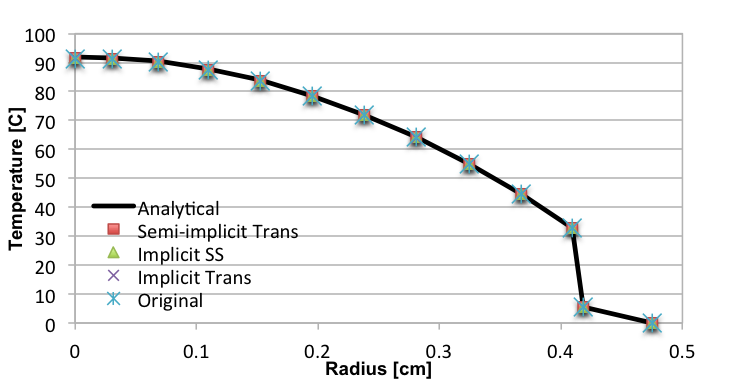
\includegraphics[width=0.60\textwidth]{images/Rod_Profile_Summary.png}
	\caption{Steady State Radial Temperature Distribution Difference to Rod Surface Temperature }
	\label{fig:Rod_Profile_Summary}
\end{figure}

\begin{figure}[!h]
	\centering
	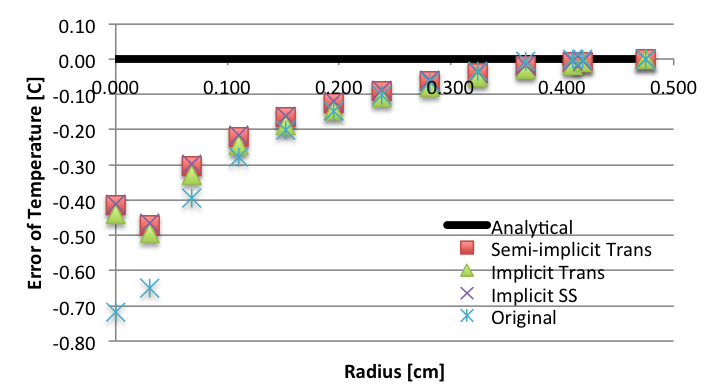
\includegraphics[width=0.60\textwidth]{images/Rod_Profile_Errors.png}
	\caption{Error of Different Numerical Methods to Analytical Solution}
	\label{fig:Rod_Profile_Errors}
\end{figure}

The relative error given in Table \ref{table:heating:errors} is shown to
scale with the inverse of the number of radial nodes in the fuel. The relative error does not scale with heat
flux, but the temperature gradient from the fuel centerline to the rod wall
does. The numerical error will also change for non-uniform heating and variable
material properties within the fuel. The implicit transient solution method has
slightly higher numerical error than the semi-implicit transient and implicit
steady state solution methods. However, all three residual formulation methods
have lower numerical error compared to the original steady state method from
CTF. The order of accuracy is difficult to compute, since CTF uses non-uniform
meshing near the rod center and since the fuel centerline temperature is
extrapolated using a second order accurate method. The non-uniform mesh size
also means that a Richardson extrapolation is not valid.

\begin{table}[h]
\center
\caption{Relative Error of Difference Between Fuel Centerline to Rod Surface Temperature}
\label{table:heating:errors}
\begin{tabular}{|c|c|c|c|c|}
\hline
NR &	SI Trans	&	I Trans	& I SS & Original SS	\\ \hline
5  & 1.33 $ \% $ & 1.35$ \% $ & 1.32$ \% $ & 2.15$ \% $ \\ \hline
10 & 0.45 $ \% $ & 0.48$ \% $ & 0.45$ \% $ & 0.78$ \% $ \\ \hline
20 & 0.15 $ \% $ & 0.18$ \% $ & 0.14$ \% $ & 0.20$ \% $ \\ \hline
\end{tabular}
\end{table}


While there is on solid conduction in the axial direction, the fluid will have a
temperature gradient in the axial direction. This will cause a 2-D temperature
distribution as shown by Figure \ref{fig:Rod_Profile}. The fluid temperature
only changes by about 10 $^{\circ}C$ from the inlet to the outlet, but the fuel
temperature changes by about 90 $^{\circ}C$ from the outer surface of the
cladding to the fuel centerline temperature. The hottest location of the fuel
is located on the centerline at the top of the rod. The centerline fuel
temperature is slightly under predicted by both the residual formulation and
the original versions of CTF. However as table \ref{table:heating:errors}
shows, this is attributable to numerical error.

\begin{figure}[!h]
	\centering
	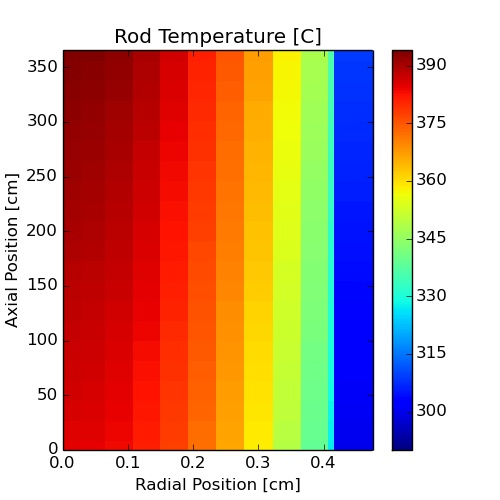
\includegraphics[width=0.60\textwidth]{images/rod_profile.jpg}
	\caption{Steady State Axial and Radial Temperature Distribution in the Fuel Rod}
	\label{fig:Rod_Profile}
\end{figure}


\section{Transient Results}

The transient simulations were run for 30.0 seconds to reach a pseudo-steady
state condition. The rate of change of the temperatures have reached near steady
state conditions as shown by Figure 7 were the red lines are fuel node
temperatures, and the black lines are cladding node temperatures. The
semi-implicit method is used on the left, and the fully implicit method is on
the right. For the semi-implicit solution method, a maximum time step size of
0.02 sec was needed to ensure stability. For the implicit solution method time
step sizes well over 0.2 seconds could be taken. For the data in the figure,
time steps of 1.0 second were used. The implicit Jacobian matrix is stiffer than
the Jacobian matrix for the semi-implicit method and therefore takes longer to
solve. Additionally, for time steps with large residuals multiple up to 5
iterations are needed. However the advantage of being able to take significantly
longer time steps makes up for the increased computational cost per time step
required by the semi-implicit method. The temperatures gained from the
semi-implicit method and the implicit methods do not differ by significant
amounts.

\begin{figure}[!h]
	\centering
	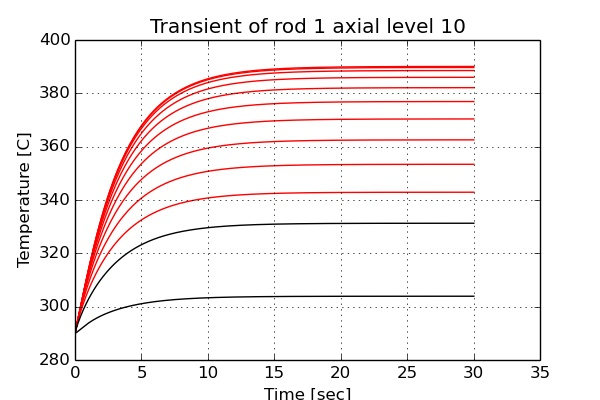
\includegraphics[width=0.60\textwidth]{images/trans_rod1_axial10_SI.jpg}
	\caption{Plot of the Radial Nodal Temperatures for the Semi-Implicit Method}
	\label{fig:trans_rod1_axial10_SI}
\end{figure}

\begin{figure}[!h]
	\centering
	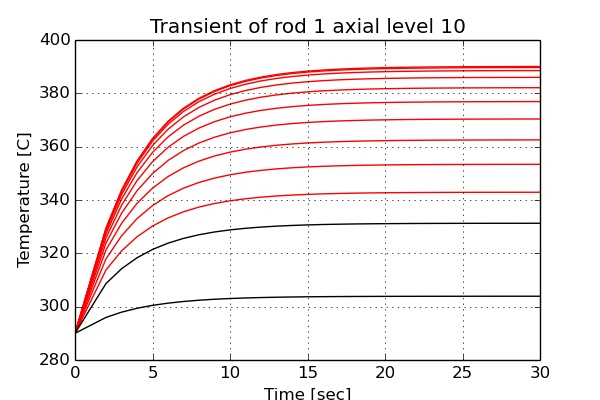
\includegraphics[width=0.60\textwidth]{images/trans_rod1_axial10_I.jpg}
	\caption{Plot of the Radial Nodal Temperatures for the Implicit Method}
	\label{fig:trans_rod1_axial10_I}
\end{figure}

The transient behavior of temperature profile is shown in Figure 8 where the
flat green line is the initial condition, the red line is the final profile, and
the black lines are intermediate time steps. It is easier to observe the
difference in the number of time steps between the semi-implicit method on the
left and the implicit method on the right. The intermediary time steps are still
the same, as is the final solution. However, the implicit method will have
greater numerical error compared to the semi-implicit method.

\begin{figure}[!h]
	\centering
	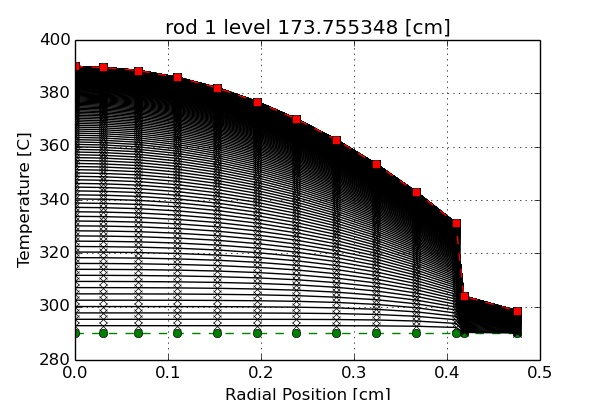
\includegraphics[width=0.60\textwidth]{images/profile_rod1_level_10_SI.jpg}
	\caption{Temperature profile over time for the Semi-Implicit Method}
	\label{fig:profile_rod1_level_10_SI}
\end{figure}

\begin{figure}[!h]
	\centering
	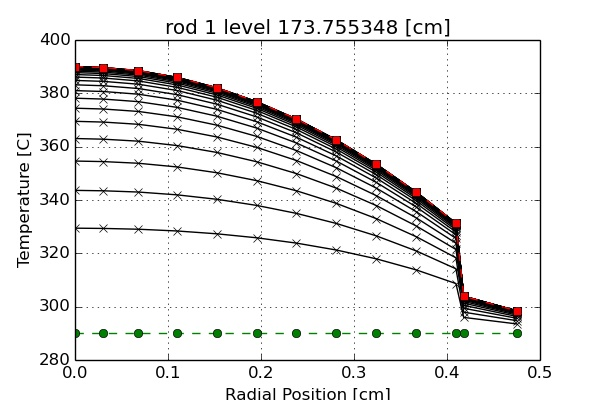
\includegraphics[width=0.60\textwidth]{images/profile_rod1_level_10_I.jpg}
	\caption{Temperature profile over time for the Implicit Method}
	\label{fig:profile_rod1_level_10_I}
\end{figure}











